\chapter{Preliminary experiments}

We will first perform some experiments using some simple models. These will
both serve as demonstrations that learning is feasible, and as baselines to
which we will compare results using more complex models. In addition, we are
comparing the performance of different kinds of input. We use both tokens,
character \ngrams and \ac{POS} \ngrams as inputs.


\section{Preprocessing}

The data files in the ASK corpus are in \ac{XML} format, and contain
information about tags, mistakes and corrections, paragraphs, sentences and
more. These files were transformed into several other formats during the
process. First, they were converted to plain text files, stripped of all tags
or correction labels. The text files have one sentence per line, consisting
of space-separated tokens, and an empty line separating paragraphs.

These raw text files were then sent through the UDPipe pipeline
\autocite{udpipe:2017} for tagging and dependency parsing. The UDPipe project
maintains an online REST \ac{API} containing a selection of pre-trained
models. All documents were transformed by the REST \ac{API} using what was at
the time of writing the newest Norwegian bokmål (nb) model
available\footnote{\texttt{norwegian-bokmaal-ud-2.3-181115}}.

The pipeline accepts raw text files as input, where each sentence is put on a
separate line. The output from UDPipe is in the CoNLL file format, with a
single token per line. UDPipe tags the documents using the Universal
Dependencies (UD) tagset, referred to as UPOS. The original tags in the ASK
corpus are from the Oslo-Bergen tagger's own tagset \autocite{oslobergen}.


\section{Metrics}
\label{metrics-discussion}

The \FI score for a single class is the harmonic mean of the precision and
recall (Eq. \ref{eq:precision}). It can also be expressed as a function of
true positives ($TP$), false negatives ($FN$), and false positives ($FP$), as
in equation \ref{eq:fscore}.

\begin{gather}
  \begin{aligned}\label{eq:precision}
    precision = \frac{TP}{TP + FP} \qquad recall = \frac{TP}{TP + FN}
  \end{aligned}
  \\[2ex]
  F_1 = 2\cdot\frac{precision\cdot recall}{precision+recall}
      = {\frac{2\cdot TP}{2\cdot TP + FN + FP}}\label{eq:fscore}
\end{gather}

In a multi-class prediction setup, there are several ways to combine the
classes' individual \FI scores into a single metric. There is the micro
average \FI, which in our case is equivalent to accuracy, since all samples
have exactly one true label. Accuracy is the proportion of samples where the
gold labels and predicted labels are the same. Then there is the macro
average, which is the unweighted average of \FI scores for all classes.

When the distribution of classes is uneven, a macro average will give
proportionally more weight on samples from small classes, and less weight to
all samples in classes with large support. A model with a high micro \FI and
a low macro \FI indicates that it is good at classifying examples from the
most frequent classes, but performs worse on classes with low support. In
addition, the weighted \FI is a weighted average where each class is weighted
proportionally to its prevalence.

\FI scores previously reported in \ac{AES} literature include Micro \FI score
in \textcite{vajjala17}, and weighted \FI in
\textcite{vajjala18universalCEFR}. For the \ac{NLI} task, micro \FI is
reported in \textcite{malmasi15,malmasi17}. Other, non-\FI metrics that have
been reported in \ac{AES} literature include \ac{QWK} \autocite{taghipour16,
alikaniotis2016automatic}, Pearson's correlation coefficient
\autocite{vajjala17, alikaniotis2016automatic}, Spearman's rank correlation
coefficient and root mean squared error \autocite{alikaniotis2016automatic},
and mean absolute error \autocite{vajjala17}. These are metrics that may
depend on the ordinal nature of proficiency scores, and potentially the
relative differences between different scores. For instance, a prediction of
`C1' for an essay with gold label `B1' is a more serious misclassification
than a prediction of `A2/B1' for the same sample, and this can be taken into
account by some metrics.

According to \textcite{yannakoudakis2015evaluating}, there are several
problems with using \ac{QWK} as a metric for the task, because it depends on
trait prevalence, the scoring scale and the marginal distributions of labels
and predictions. Therefore it is problematic to compare \ac{QWK} scores
between different systems and datasets. However, since two of the cited
studies are based on a dataset from a Kaggle competition where \ac{QWK} was
the official metric, it has been reported.


\subsection{Reported metrics}

We report both the macro and micro \FI for all experiments. The metrics are
reported for two different modes: The first utilizing the full set of
classes, and the second training and evaluating on the collapsed classes.

A third option, namely to train on the full set of classes and reduce the
predictions to the collapsed set of classes, was also attempted, based on the
assumption that the more fine grained labels in the full set of classes can
provide useful supervision signals even though we evaluate on a smaller set.
However, in practice the best performers on the collapsed labels was
empirically observed to be the models that were also trained on the collapsed
tags.


\section{Model descriptions}

Initial experiments were run using linear models, logistic regression,
and linear regression, and neural models following the \acp{MLP} architecture.


\subsection{Classification versus regression}

\ac{AES} can be modelled both as a classification task and as a regression
task, and both are seen in previous work.

A disadvantage with using regression for the AES task is that while we know the
correct order of classes, it is not obvious that the distance between adjacent
classes is always equal. For instance, we cannot know if the jump from CEFR
score `A2/B1' to 'B1' is just as big as `B1' to `B1/B2'. However, we need to
implicitly decide this when we transform the labels into numeric values for
regression.

This challenge of quantifying distance between classes does not apply to the
classification approach, but it comes with another problem. Multi-class
classification does not consider any ordering of classes, which is an
intrinsic property of the classes for AES.

A third class of analysis called \emph{ordinal regression} or \emph{ranking
learning} is intended for predicting an ordinal variable, such as CEFR scores.


\subsection{Input representations}

Input representations are shared between the linear and neural models, except
for the total number of features. The neural models may restrict the number
of features by cutting off less frequently occurring features, and this is
noted below.

\subsubsection*{Word counts}

This representation is a vector with a entry for each unique word form in the
training data, 20,766 in total. The value of each entry is the number of
times the word form occurs in the document. The neural models limits the
count vectors to the 10,000 most common tokens.

\subsubsection*{Character \ngrams}

Documents are represented by count vectors where each entry represents a
\ngram of characters. Some examples of character \ngrams are
$\langle$eg␣$\rangle$, $\langle$␣i␣$\rangle$ or $\langle$si$\rangle$. For the
linear model, all \ngrams with $n\in \{1,2,3\}$ were used, and for the neural
models the 10,000 most commonly occurring \ngrams with $n\in \{2,3,4\}$ were
used.

\subsubsection*{POS \ngrams}

Documents are represented by count vectors where each entry represents a
\ngram of POS tags. Some examples of POS \ngrams are $\langle$NOUN
NOUN$\rangle$, $\langle$PRON AUX PRON$\rangle$ or $\langle$SCONJ
ADJ$\rangle$. For the linear model, all \ngrams with $n\in \{1,2,3\}$ were
used, and for the neural models the 10,000 most commonly occurring \ngrams
with $n\in \{2,3,4\}$ were used.

\subsubsection*{Mixed POS}

The Mixed POS mode was taken from \textcite{malmasi15}. Their best performing
single feature was a mix of word forms and POS tags, so that common function
words appeared in their written form, while content words were substituted
with their POS tag.

\begin{example}
% cSpell:disable-next
\gll generasjoner kan også få   anledning til å utnytte dem  
% cSpell:disable-next
     NOUN         kan også VERB NOUN      til å VERB    dem  
\glt `generations can also have the opportunity to exploit them'
\glend
\label{ex:mixed-pos}
\end{example}

Example \ref{ex:mixed-pos} shows a sentence fragment with the original series
of tokens, the sequence of mixed function words and UPOS tags it is
transformed into, as well as a translation into English.

The \ngram features add a certain sensitivity to local order of features.
Many character \ngrams will represent entities smaller than a word, but may
indicate common spelling mistakes. \ac{POS} and Mixed POS \ngrams, on the
other hand, might be able to represent syntactic features. Spelling and
syntax should be correlated with L2 proficiency, and traditional \ac{ML}
methods that rely on manual feature engineering have included domain specific
features designed to capture spelling and syntax, as for instance in
\textcite{vajjala17}.

We used the same set of stop words as \citeauthor{malmasi15}. From these
transformed sequences, we extracted \ngrams in the interval $[1,3]$. The
20,000 most commonly occurring of these were used for the neural models.


\subsection{Linear models}
\label{subsec:linear}

The logistic regression model was implemented using the Python library
Scikit-Learn \autocite{scikit-learn}. The model was instantiated with the
`lgbfs' solver to minimize multinomial loss. No regularization was used, and
the optimizer was set to run for a maximum of 100 iterations.

The linear regression model was a support vector regressor
also chosen from Scikit-learn. The default
parameters were used, which 

In order to report classification based metrics for a regression model, we
had to transform the predicted scores, which are continuous, into discrete
scores equivalent to the given classes. This was by rounding the raw
regression score to the nearest integer and clipping the result to be in the
range of the highest and lowest classes.


\subsection{Multi-layer perceptron}
\label{subsec:mlp}

The MLP models were implementing in Keras \autocite{keras} and run on the
TensorFlow backend \autocite{tensorflow}. All the models the have an input
layer with 20,000 dimensions, followed by two fully connected layers with 100
and 300 nodes, respectively. The fully connected layers use \ac{ReLU}
activation and dropout regularization with a dropout rate of 50\%.

The output layer varies depending on the method used. For multi-class
prediction, we use an output layer with softmax activation and 7 or 4
dimensions, depending on whether we run with collapsed labels or not. The
multi-class model was trained by minimizing the categorical cross-entropy
loss (Eq. \ref{eq:crossentropy}).

For regression, our output layer contains a single node with sigmoid
activation. The regression model is trained by minimizing the mean squared
error loss against gold labels normalized to the interval $[0, 1]$. This is
in line with the method for neural network regression used by
\textcite{taghipour16}. For evaluating the predictions, the output is scaled
by the value of the highest label and transformed into categorical values
using the method described in subsection \ref{subsec:linear}.

The codomain of sigmoid function is centered around 0.5 and maps to the
central labels. The highest and lowest labels get a smaller share of the
space.

For ordinal regression, we implemented a neural model for ordinal regression
following a modified version of the method in \textcite{cheng2008neural}.
Gold labels are represented as a vectors of size $C-1$ where the elements are
filled with ones from left to right such that: The lowest class is all zeros.
The next class is a single one in the leftmost position and zeros in the
remaining positions. The next class has two ones in the two leftmost
positions, continuing to the highest class which is represented by a vector
of only ones. In the original paper, \citeauthor{cheng2008neural} used
vectors of size $C$. However, we only need $C-1$ elements to represent the
thresholds between classes.

The output layer of our neural network has size $C-1$ and uses elementwise
sigmoid activation to constrain the values of elements to the interval
$(0,1)$. At train time, we minimize the mean square error between the gold
labels and output.

At predict time, we apply a rounding function to the output vectors such that
we get a vector of only ones and zeros. The resulting vector may be any
sequence of ones and zeros, even those not conforming to our rule for
representing classes, i.e. there might be a one to the right of a zero. We
then select the predicted class by taking the index of the first zero element
of this vector, or the highest class if all elements are one.

The multi-class and ordinal regression neural networks were trained using the
Adam optimization algorithm \autocite{kingma2014adam} with a learning rate of
$2\cdot 10^{-4}$. The neural regressor was trained with the RMSProp
optimization algorithm.


\section{Results}

Two different sets of output labels are used in the experiments: The original
seven CEFR labels, and a collapsed set where the intermediate classes, such
as ``A2/B1'', are rounded up to the nearest canonical class, i.e. the CEFR
label after the slash. This results in only four different labels: ``A2'',
``B1'', ``B2'' and ``C1''. All macro and micro \FI scores for the classifiers
described in this chapter, for both the full and collapsed sets of classes,
are found in table \ref{tab:baseline-accuracies}.

\begin{table}
  \centering
  \begin{tabular}{lrrrr}
    \toprule
             & \multicolumn{2}{c}{All labels} & \multicolumn{2}{c}{Collapsed labels} \\
    \cmidrule(lr){2-3}
    \cmidrule(lr){4-5}
    Model      & Macro \FI & Micro \FI & Macro \FI & Micro \FI \\
    \midrule
    Majority   &  $0.040$  &  $0.163$  &  $0.127$  &  $0.341$ \\
    \midrule
    % $BEGIN autotable baseline-accuracies
    % $META models-per-row=2 columns-per-model=macrof1,microf1
    % $ROW LogReg BOW: linear_logreg-1337_1 linear_logreg-1338_1
    % $ROW LogReg Char: linear_logreg-1337_2 linear_logreg-1338_2
    % $ROW LogReg POS: linear_logreg-1337_3 linear_logreg-1338_3
    % $ROW LogReg Mix: linear_logreg-1337_4 linear_logreg-1338_4
    % \midrule
    % $ROW SVC BOW: linear_svc-1337_5 linear_svc-1338_5
    % $ROW SVC Char: linear_svc-1337_6 linear_svc-1338_6
    % $ROW SVC POS: linear_svc-1337_7 linear_svc-1338_7
    % $ROW SVC Mix: linear_svc-1337_8 linear_svc-1338_8
    % \midrule
    % $ROW SVR BOW: linear_svr-1337_9 linear_svr-1338_9
    % $ROW SVR Char: linear_svr-1337_10 linear_svr-1338_10
    % $ROW SVR POS: linear_svr-1337_11 linear_svr-1338_11
    % $ROW SVR Mix: linear_svr-1337_12 linear_svr-1338_12
    % \midrule
    % $ROW MLP BOW:    mlp_bow-26436597_13 mlp_bow-26436607_13
    % $ROW MLP Char:   mlp_char-26436597_14 mlp_char-26436607_14
    % $ROW MLP POS:    mlp_pos-26436597_15 mlp_pos-26436607_15
    % $ROW MLP Mix:    mlp_mix-26436597_16 mlp_mix-26436607_16
    % \midrule
    % $ROW MLP Reg BOW:    mlp_bow-26436597_17  mlp_bow-26436607_17
    % $ROW MLP Reg Char:   mlp_char-26436597_18 mlp_char-26436607_18
    % $ROW MLP Reg POS:    mlp_pos-26436597_19  mlp_pos-26436607_19
    % $ROW MLP Reg Mix:    mlp_mix-26436597_20  mlp_mix-26436607_20
    % \midrule
    % $ROW MLP Rank BOW:   mlp_bow-26449272_21  mlp_bow-26449273_21
    % $ROW MLP Rank Char:  mlp_char-26449272_22 mlp_char-26449273_22
    % $ROW MLP Rank POS:   mlp_pos-26449272_23  mlp_pos-26449273_23
    % $ROW MLP Rank Mix:   mlp_mix-26449272_24  mlp_mix-26449273_24
    % $END autotable
    LogReg BOW & $0.199$ & $0.317$ & $0.384$ & $0.626$ \\
    LogReg Char & $0.221$ & $0.317$ & $0.399$ & $0.602$ \\
    LogReg POS & $0.190$ & $0.301$ & $0.312$ & $0.569$ \\
    LogReg Mix & $0.213$ & $0.341$ & $0.337$ & $0.577$ \\
    \midrule
    SVC BOW & $0.210$ & $0.317$ & $0.391$ & $0.610$ \\
    SVC Char & $0.189$ & $0.293$ & $0.347$ & $0.537$ \\
    SVC POS & $0.157$ & $0.244$ & $0.336$ & $0.618$ \\
    SVC Mix & $0.215$ & $0.350$ & $0.319$ & $0.585$ \\
    \midrule
    SVR BOW & $\mathbf{0.444}$ & $0.415$ & $0.429$ & $0.659$ \\
    SVR Char & $0.252$ & $0.317$ & $0.440$ & $0.602$ \\
    SVR POS & $0.334$ & $0.358$ & $\mathbf{0.476}$ & $0.593$ \\
    SVR Mix & $0.312$ & $0.350$ & $0.441$ & $0.659$ \\
    \midrule
    MLP BOW & $0.252$ & $0.398$ & $0.382$ & $0.659$ \\
    MLP Char & $0.264$ & $0.415$ & $0.417$ & $0.675$ \\
    MLP POS & $0.237$ & $0.407$ & $0.393$ & $0.642$ \\
    MLP Mix & $0.232$ & $0.398$ & $0.353$ & $0.659$ \\
    \midrule
    MLP Reg BOW & $0.246$ & $0.341$ & $0.458$ & $\mathbf{0.715}$ \\
    MLP Reg Char & $0.286$ & $0.341$ & $0.468$ & $0.707$ \\
    MLP Reg POS & $0.273$ & $0.390$ & $0.418$ & $0.699$ \\
    MLP Reg Mix & $0.252$ & $0.423$ & $0.440$ & $0.650$ \\
    \midrule
    MLP Rank BOW & $0.276$ & $0.398$ & $0.408$ & $0.707$ \\
    MLP Rank Char & $0.330$ & $\mathbf{0.480}$ & $0.395$ & $0.634$ \\
    MLP Rank POS & $0.251$ & $0.382$ & $0.420$ & $0.667$ \\
    MLP Rank Mix & $0.235$ & $0.366$ & $0.403$ & $0.634$ \\
    \bottomrule
  \end{tabular}
  \caption{\FI scores of different classifiers}
  \label{tab:baseline-accuracies}
\end{table}

As a simple baseline, we consider the majority class classifier. The majority
class in the training set is ``B1'', both with the full class set of labels
and with the collapsed set. The macro \FI scores for the majority classifier
are very low, as the majority class classifier predicts no samples for any
classes except the majority, and thus the \FI score for all other classes is
zero\footnote{Technically, the precision is undefined when there are no
predictions for the class, but it is commonly set to 0 in this case.}.


\subsection{Linear models}

Moving to a linear model, a logistic regression classifier (LogReg) using
bag-of-words features achieves a macro \FI score of 19.9\% on the dev set
without collapsed labels and 38.4\% with collapsed labels, and thus beats the
majority classifier by a large margin. However, the classifier performs
better using another input representation than bag-of-words. Character
\ngrams yields the highest macro \FI scores using a logistic regression
classifier, 22.1\% and 39.9\% for all classes and collapsed classes,
respectively.

The \ac{SVM} classifier, referred to as SVC in the table, performs around the
same level as the LogReg classifier. Its highest macro \FI scores, 21.5\% and
39.9\%, are lower than for LogReg.

The \ac{SVM} regressor, referred to as SVR, improves on all macro \FI scores
from the linear classifiers, and also has the highest micro \FI scores of all
the linear models. Using bag-of-words input, the model yields a macro \FI of
44.4\% on the full set of labels. For the collapsed set of labels, the highest
macro \FI, 47.6\%, comes from POS \ngram features.


\subsection{Neural networks}

However, our \acp{MLP} had the best accuracies. For the full set of
classes, character \ngrams gave the best results, followed by POS \ngrams.
For the collapsed classes, POS \ngrams outperformed character \ngrams by a
small margin. Interestingly, the input representation that yielded the best
scores in our linear models, mixed UPOS, did not give good results with the
\acp{MLP} at all. This may indicate that the neural model is able to extract
higher-level features that model the interaction between several low-level
\ngram features.

In order to examine the classification behaviour closer, we present the
confusion matrices from MLP Mix in figures \ref{fig:mlp-mixed-conf} and
\ref{fig:mlp-mixed-conf-round}. We want predictions to lie on the diagonal of
the matrix. However, due to the ordinal nature of the classes, we also want
eventual misclassifications to lie close to the diagonal, as would indicate a
small magnitude of misclassification. Conversely, we do not want any
predictions in the upper right and lower left corners, as they represent
misclassifications of the greatest magnitude.

\begin{figure}
  \centering
  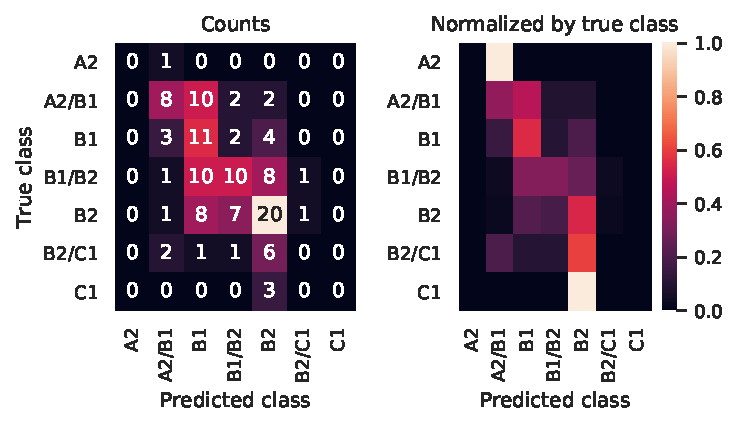
\includegraphics{mlp-mixed-conf}
  \caption{Confusion matrix for MLP Mix}
  \label{fig:mlp-mixed-conf}
\end{figure}

\begin{figure}
  \centering
  \includegraphics{mlp-mixed-conf-round}
  \caption{Confusion matrix for MLP Mix on collapsed labels}
  \label{fig:mlp-mixed-conf-round}
\end{figure}
